\documentclass[12pt]{article}
\usepackage{graphicx}
\usepackage{amsmath}
\usepackage{amssymb}
\usepackage{color}
\usepackage{caption}
\usepackage{subcaption}
\usepackage{mdframed}
\usepackage[margin=3cm]{geometry}
\usepackage[superscript,nomove]{cite}
\numberwithin{equation}{section}
\numberwithin{figure}{section}
\usepackage[makeroom]{cancel}
\usepackage{textcomp}
\usepackage{gensymb}
\DeclareMathOperator\arctanh{arctanh}
\usepackage[colorlinks=true]{hyperref}
\usepackage{cleveref}
\crefdefaultlabelformat{[#2#1#3]}
\begin{document}
\renewcommand\citeform[1]{[#1]}
%
\title{MSc Data Science Project: Can a Convolutional Neural Network judge a book by its cover?}
\author{\\Ryan Hill MSci\\\\
Supervisor: Dr Hubie Chen\\\\
Birkbeck, University Of London\\\\
\texttt{rhill06@mail.bbk.ac.uk}}
\date{\today}
\maketitle
\thispagestyle{empty}
\graphicspath{{images/}}
\begin{abstract}
	Coming soon...
\end{abstract}
\begin{figure}[!b]
	\centering
	
\includegraphics[scale=0.4]{bbk_logo.jpg}
\end{figure}

\clearpage
%
{\hypersetup{linkcolor=black}
\tableofcontents}
\thispagestyle{empty}
\clearpage
%
\setcounter{page}{1}
\section{Introduction} 
\label{sec:intro}

Introduce the project, describe the goal and the idea behind why this is important. Explain the structure of this work,


In this work we will use the terms \emph{class, genre, classification,} and \emph{category} interchangeably to describe the genre that a particular book cover belongs to.
\subsection{Related Works} 
\label{sub:Related Works} 
Discuss the work of Iwana as the main source, reference their methods and results but keep much for later where relevant for comparison with my work.
% subsection Related Works end 
% section CNN Theory and Architectures
\section{Theory} 
\label{sec:Theory} 
\subsection{Components of Convolutional Neural Networks} 
\label{sub:Components_of_Convolutional_Neural_Networks} 
Describe the maths and the theory behind the various components of CNNs to the best of my ability, referring to the source papers for more complex combined units where sensible. 
% subsection Components_of_Convolutional_Neural_Networks end 
\subsection{Transfer Learning} 
\label{sub:Transfer_Learning} 
Describe the theory and maths behind transfer learning to the reader.
% subsection Transfer_Learning end 

\subsection{Activation Maximisation} 
\label{sub:Activation_Maximisation} 
Describe the theory and/or maths of activation maximisation and the methods used within the package we use the regularisations applied. 
% subsection Activation_Maximisation end 
% section Theory end 
\section{Data collection and pre-processing} 
\label{sec:Data_collection_and_pre-processing} 
\subsection{Image Download and Manual Review} 
\label{sub:Image Download and Manual Review} 
The 207, 572 images within the complete book32 dataset covering all original 32 classes were downloaded at full resolution using a slightly altered version of the script provided within the Iwana repository \cite{iwanarepo}. The original csv containing all image URLs was split into files of no more than 20,000 records each to allow to the downloads to be run over multiple sessions do to the slow data transfer rates and the overhead of reading data between Google Drive and Google Colab meaning that even checking before downloading an individual file was not much faster than downloading and writing the file anyway. Each sub-file was then iterated over using the remainder of the original script, downloading each image into a sub-folder of the class for that image i.e. the genre classification.

Once all images were downloaded a sample few were manually checked to verify as best as possible that the data was still correct and the downloads has worked. At this point we attempted to identify if any records used in the bookcover30 train or test datasets were actually boxsets, and as such would likely have an unrepresentative cover image, and example of such an image can be seen in \textcolor{red}{TODO: add image}\cref{fig:TBC}. The terms used in a regex search of the titles were \emph{"boxed set", "boxset", "box set", "anthology", "bundle", "\#-book", "\# book"}. 264 records within the bookcover30 dataset matched at least one of these terms and were extracted into a new folder for manual review. The process was somewhat subjective but as a rule of thumb we rejected any image that was not a single front facing cover, that contained pictures of multiple books and was not an arrangement of covers; single covers that seemed to be specifically designed for a boxset were considered acceptable. In total 94 records needed to be removed due to these rules. To preserve the class balance of the train and test datasets, new records were chosen from the book32 dataset by making like-for-like swaps of the same class; any new covers were also reviewed to ensure they were not boxsets. No verification of the class assignment to images was performed so any errors that existed in the original data would have persisted and we continue to use the single class chosen by the original authors in the case of multi-class books.

We chose to split the training data out into training and validation data using a 90/10 random split per class to ensure class balance in all of the training, validation, and test sets. In total the training set compromised of 46,170 records, the validation set 5130 records, and the test set 5700 records; with 1,539, 171, and 190 records per class respectively. 

% subsection Image Download and Manual Review end 
\subsection{Image Pre-processing Technique} 
\label{sub:Image_Pre-processing_Technique} 

We next used 3 different image preparation methods on the datasets to attempt to identify the method that would lead to the best accuracy within our models. At this stage all methods output an image 299x299 pixels as this was the largest size we would need for any future models. By reducing the image size twice, first now and then again when using a specific model, we were potentially losing some information that would lead to a less accurate model; however we chose to do this to speed up training and testing by having to load much smaller data in compared to the original full sized images. Before pre-processing was done we collected the initial shape and average RGB values of each image for further analysis later.

The first pre-processing method (\emph{NoPrep}) was to simply rescale the image directly down to a 299x299 shape using inter-cubic interpolation \textcolor{red}{TODO: explain this mathematically}. This was chosen at the time as a common all-purpose interpolation method, however after later research this method is often chosen to enlarging images, not shrinking them so the potential to use a better interpolation method could be used in future work.

The second method (\emph{Padded}) was to first pad the images with a symmetric pure white border on either the left/right or top/bottom depending on if the image was portrait or landscape (no padding was done if the image was already a perfect square). These images were then downscaled to 299x299 using the same method as above. The final method (\emph{Cropped}) was to crop the image to a perfect square before the same downscaling method was used. 

Once the images had been processed we used a MobileNetV2 model on each processed training and validation dataset for 30 epochs with an early stopping patience of 15 (i.e. if no improvement was seen in validation accuracy over 15 epochs then we did not continue) and the best model for validation accuracy was kept. The model was trained using the default TensorFlow 2 settings of the adam optimiser with a loss function of sparse categorical cross entropy. More details of the set up are detailed in \cref{sec:Model_Training} as other than the epoch and early stopping the same configuration was used for the main training process. The progress on the training and validation data can be seen in \cref{fig:prep_perf} and the test results of this model trained on each of the 3 datasets is presented in \cref{tab:preprocres}. The second method, padding the image with a white border, achieved the best result on the test data of 15.81\% accuracy. 

\begin{figure}
	\centering
	\captionsetup{justification=centering}
	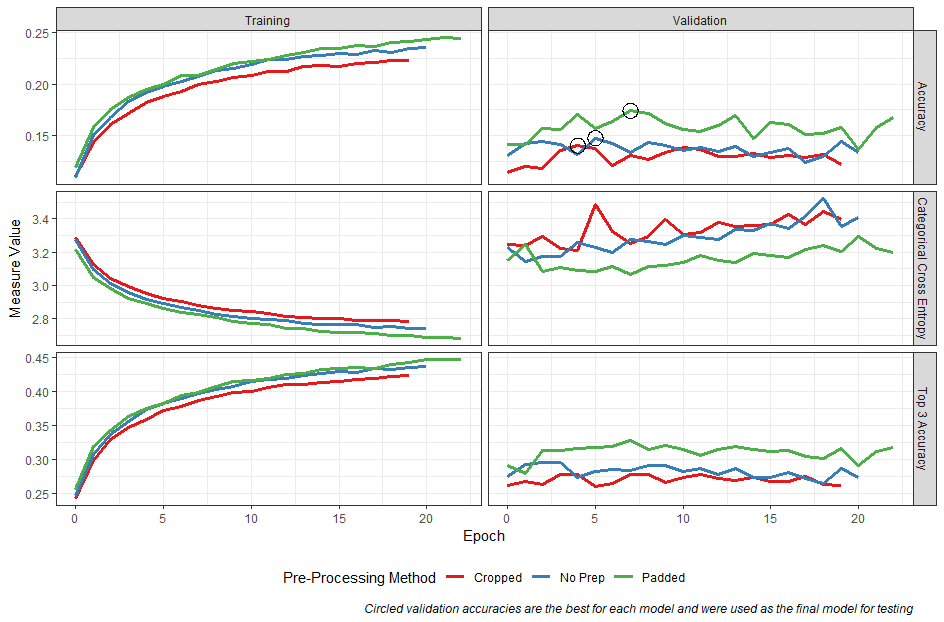
\includegraphics[scale=0.5]{prep_training.png}
	\caption{Performance of different pre-processing methods throughout training of MobileNetV2}
	\label{fig:prep_perf}
\end{figure}


\begin{table}[]
	\centering
	\begin{tabular}{|l|r|r|}
	\hline
	\textbf{Pre-processing Method} & \multicolumn{1}{l|}{\textbf{Best epoch}} & \multicolumn{1}{l|}{\textbf{Test Accuracy}} \\ \hline
	NoPrep                         & 8                                        & 14.39\%                                     \\ \hline
	Padded                         & 6                                        & 15.81\%                                     \\ \hline
	Cropped                        & 5                                        & 12.88\%                                     \\ \hline
	\end{tabular}
	\caption{Results of short training on MobileNetV2 on different image pre-processing methods}
	\label{tab:preprocres}
\end{table}

It is important to note at this point that just because this method achieved the best result for this model in a short number of epochs is no guarantee that this would be the method that achieves the best results in other models or over longer epochs. We use this as a rough benchmark as given the constraints on computing power available to us we were only able to train each model in \cref{sec:Model_Training} once for a reasonable number of epochs, so a decision had to be made. It is also possible that hyperparameter tuning for each of these datasets may have led to different outcomes, but again due to the constraint on resources we decided it best to use domain accepted defaults and as such we progress with the padded dataset.

% section Image_Pre-processing_Technique end 
% section Data_Collection_and_pre-processing end 
\section{Model Training} 
\label{sec:Model_Training} 
\subsection{Configuration} 
\label{sub:Configuration} 
All model architectures consisted of their respective base CNN structure as detailed in \cref{sec:CNN_Architectures} followed by a global average pooling 2D layer to reduce the dimensionality of our tensor and to ensure a flat 1D vector which is fully connected to a 30 neuron output layer with a softmax activation. All models were also trained using the same setup in terms of hyperparameters, optimisers and loss functions; the loss function was sparse categorical cross entropy (sparse due to the usage of a non one-hot encoded target vector), the optimiser was the Adam optimiser \cite{Kingma2015}. The optimiser was used with default hyperparameters as defined within the TensorFlow implementation, the most important being the learning rate with was left at the initial value of 0.001. The reason for the usage of the default hyperparameters and not using a more advanced custom optimiser, such as WAME \cite{Mosca2017}, was due to the constraints on access time to computing power. As is the training already had to be completed across multiple sessions and doing any tuning would have resulted in too large a time required to produce meaningful results; Adam produces decent results with the defaults and so they were used in this work.

The models themselves, MobileNetV2, Inception-ResnetV2, and ResNeXt50 were chosen to represent a wide spread of model capabilities and complexities as highlighted in Figure 1 of the Benchmark Analysis of CNNs completed by Bianco et al\cite{Bianco2018}. MobileNetV2 was chosen as it is a lightweight model designed to be capable of running on mobile devices and was meant to be a low complexity comparison in line with AlexNet (due to no pre-trained version of AlexNet being available within TensorFlow), Inception-ResnetV2 for its high accuracy in other use cases, and ResNeXt50 as a smaller version of one of the newer CNN architectures. These models, combined with the original work done by Iwana et al, span a range of complexity and training speed allowing for a good comparison between performance.

The models were training once using the training data as described in \cref{sub:Image Download and Manual Review} and validated against the validation data split out at the same point. No cross-validation was done due to resource limitations.
% subsection Configuration end 
\subsection{Training Performance} 
\label{sub:Training_Performance} 
The models were each trained with a maximum of 200 epochs and early stopping with a patience of 20 due to the time constraints; in the end all 3 models resulted in early stopping by epoch 104 at most. 

The performance of the models throughout training can be seen in \cref{fig:train_perf} where whilst training accuracy continues to increase over time, the validation accuracy doesn't see as much consistent movement which suggests the model is starting to overfit to the training data as opposed to improving the identification of intrinsic underlying features within the images themselves. Iwana does not report their training accuracy so we are not able to compare the performance of our training with theirs.

\begin{figure}
	\centering
	\captionsetup{justification=centering}
	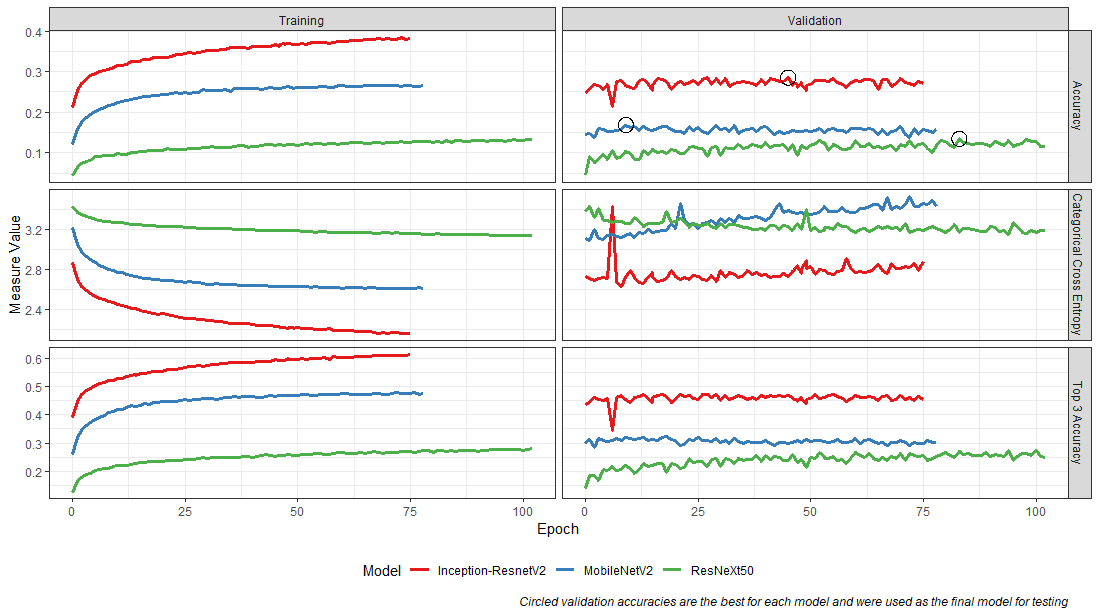
\includegraphics[scale=0.5]{training_results.png}
	\caption{Performance of models on training and validation data throughout training. Note that models that end short stopped training due to early stopping.}
	\label{fig:train_perf}
\end{figure}

Iwana et al trained their models for 30,000 and 450,000 epochs for LeNet and AlexNet respectively, substantially more than we trained our models for, so it is likely that the results they achieved are better than they would have been if they had trained for only a few hundred epochs. It is possible, but not certain, that by training our models for a factor of 10 or 100 more epochs, and removing the early stopping criteria, that we could have achieved even better validation performance. 

MobileNetV2 achieved the best validation accuracy early on in the training, where Inception-ResNeXt50 continued to see improvement until just before the 50th epoch/ ResNeXt50 sees its best performance coming after the 75th epoch, but as we will see this is not indicative of better performance the accuracy at any time never improved beyond the lowest accuracy for MobileNetV2 on the training or validation data despite being a more complex model and training for more epochs.
% subsection Training_Performance end 

% section Model_Training end 

\section{Evaluation} 
\label{sec:Evaluation_and_Further_Exploration} 
\subsection{Results} 
\label{sub:Results} 
Full results for all 3 models evaluated on the test set are available in \cref{tab:results_acc}, along with those reported by Iwana for ease of comparison. A visual representation of this for our models only is shown in \cref{fig:test_perf}. As a reminder, the dataset used for our models was slightly altered from the original set, and due to the use of a validation dataset did not contain the set of records; but for a comparison it is suitable. Inception-ResnetV2 is comparable to the results of AlexNet but is slightly more accurate when Top-3 predictions are taken into account. MobileNetV2 is close to LeNet in performance, with just slightly improvements in many genres. ResNeXt50 shows very odd behaviour, with many classes showing near 0\% accuracy even at Top-3, whilst some classes have a very high accuracy such as Biographies and Memoirs. This is likely an artefact of it overlapping specific classes which along with is discussed further in \cref{sub:Further_Analysis}.

At a per-genre level Inception-ResnetV2 shows the best results on 16 out of the 30 genres for top-1 predictions, followed by 10 for AlexNet. If we further explore the seemingly best performing classes in ResNeXt50 we can see by looking at the precision as presented in \cref{tab:test_prec} that in the genres where this model seems to perform well the precision is low (when compared to for example Inception-ResnetV2) which provides further evidence that for some classes it combines multiple genres and just predicts one of them i.e. whilst the model is able to correctly predict these \emph{chosen}	classes when it sees them, it is highly likely to predict other genres as one of these as well.

Overall the results from Inception-ResnetV2 are promising given the low training time and adjusted dataset; the potential improvements are discussed further in \cref{sub:Discussion}.

\begin{table}[]
	\centering
	\resizebox{\textwidth}{!}{%
	\begin{tabular}{lrrrrrrrrrrrrrr}
								   & \multicolumn{2}{c}{\textbf{LeNet*}}                                     & \multicolumn{1}{c}{\textbf{}} & \multicolumn{2}{c}{\textbf{AlexNet*}}                                   & \multicolumn{1}{c}{\textbf{}} & \multicolumn{2}{c}{\textbf{MobileNetV2}}                                & \multicolumn{1}{c}{\textbf{}} & \multicolumn{2}{c}{\textbf{Inception-ResnetV2}}                         & \multicolumn{1}{c}{\textbf{}} & \multicolumn{2}{c}{\textbf{ResNeXt50}}                                  \\
	\textbf{Genre}                 & \multicolumn{1}{c}{\textbf{Top 1}} & \multicolumn{1}{c}{\textbf{Top 3}} & \multicolumn{1}{c}{\textbf{}} & \multicolumn{1}{c}{\textbf{Top 1}} & \multicolumn{1}{c}{\textbf{Top 3}} & \multicolumn{1}{c}{\textbf{}} & \multicolumn{1}{c}{\textbf{Top 1}} & \multicolumn{1}{c}{\textbf{Top 3}} & \multicolumn{1}{c}{\textbf{}} & \multicolumn{1}{c}{\textbf{Top 1}} & \multicolumn{1}{c}{\textbf{Top 3}} & \multicolumn{1}{c}{\textbf{}} & \multicolumn{1}{c}{\textbf{Top 1}} & \multicolumn{1}{c}{\textbf{Top 3}} \\ \hline
	Arts \& Photography            & 5.8                                & 11.6                               &                               & 12.1                               & 31.1                               &                               & 11.1                               & 27.9                               &                               & \textit{13.2}                      & \textit{33.7}                      &                               & 3.7                                & 11.1                               \\
	Biographies \& Memoirs         & 5.3                                & 18.4                               &                               & 13.2                               & 29.5                               &                               & 10.0                               & 30.5                               &                               & \textit{23.2}                      & 46.3                               &                               & 20.0                               & \textit{60.0}                      \\
	Business \& Money              & 10.0                               & 25.3                               &                               & 12.6                               & 25.8                               &                               & 4.7                                & 18.4                               &                               & \textit{13.2}                      & \textit{33.7}                      &                               & 1.1                                & 3.2                                \\
	Calendars                      & 18.9                               & 37.9                               &                               & \textit{47.9}                      & \textit{65.3}                      &                               & 13.7                               & 25.8                               &                               & 25.8                               & 37.4                               &                               & 18.9                               & 24.7                               \\
	Children’s                     & 24.7                               & 42.1                               &                               & \textit{42.1}                      & \textit{61.6}                      &                               & 30.0                               & 52.1                               &                               & 18.9                               & 43.2                               &                               & 11.6                               & 34.7                               \\
	Comics \& Graphic Novels       & 15.8                               & 33.7                               &                               & 47.4                               & 67.9                               &                               & 40.5                               & 56.8                               &                               & \textit{56.3}                      & \textit{72.6}                      &                               & 47.9                               & 60.5                               \\
	Computers \& Technology        & 29.5                               & 42.8                               &                               & \textit{44.7}                      & \textit{59.5}                      &                               & 28.4                               & 43.7                               &                               & 41.1                               & 57.4                               &                               & 17.9                               & 26.8                               \\
	Cookbooks, Food \& Wine        & 14.2                               & 32.6                               &                               & \textit{43.7}                      & \textit{57.4}                      &                               & 23.7                               & 42.1                               &                               & 40.0                               & 55.8                               &                               & 7.9                                & 23.2                               \\
	Crafts, Hobbies \& Home        & 7.4                                & 22.1                               &                               & 17.4                               & 36.8                               &                               & 13.7                               & 30.5                               &                               & \textit{31.6}                      & \textit{60.0}                      &                               & 2.6                                & 15.3                               \\
	Christian Books \& Bibles      & \textit{8.4}                       & 23.7                               &                               & 7.4                                & \textit{26.3}                      &                               & 2.6                                & 12.1                               &                               & 4.2                                & 20.5                               &                               & 0.0                                & 0.5                                \\
	Engineering \& Transportation  & 10.0                               & 21.1                               &                               & 20.0                               & 34.7                               &                               & 15.3                               & 32.1                               &                               & \textit{20.0}                      & \textit{35.3}                      &                               & 6.8                                & 24.7                               \\
	Health, Fitness \& Dieting     & 4.2                                & 15.8                               &                               & 12.6                               & 29.5                               &                               & 4.2                                & 17.9                               &                               & \textit{12.6}                      & \textit{37.4}                      &                               & 3.7                                & 25.8                               \\
	History                        & 6.3                                & 16.8                               &                               & 12.6                               & 27.9                               &                               & 6.8                                & 21.6                               &                               & \textit{15.8}                      & \textit{38.4}                      &                               & 1.1                                & 2.1                                \\
	Humor \& Entertainment         & 5.3                                & 16.3                               &                               & 10.5                               & 22.6                               &                               & 0.0                                & 7.4                                &                               & \textit{16.3}                      & \textit{43.7}                      &                               & 0.0                                & 2.6                                \\
	Law                            & 14.7                               & 25.8                               &                               & 25.3                               & 38.4                               &                               & 16.3                               & 27.4                               &                               & 17.9                               & 37.9                               &                               & \textit{26.8}                      & \textit{45.3}                      \\
	Literature \& Fiction          & 3.2                                & 12.1                               &                               & \textit{11.1}                      & 22.6                               &                               & 6.3                                & 24.7                               &                               & 10.5                               & \textit{38.9}                      &                               & 0.5                                & 2.6                                \\
	Medical Books                  & 12.6                               & 30.0                               &                               & 19.5                               & 36.8                               &                               & 11.1                               & 27.4                               &                               & \textit{20.0}                      & \textit{45.8}                      &                               & 13.7                               & 38.9                               \\
	Mystery, Thriller \& Suspense  & 23.7                               & 40.0                               &                               & 34.2                               & 48.9                               &                               & 12.1                               & 28.9                               &                               & \textit{34.7}                      & \textit{59.5}                      &                               & 19.5                               & 28.9                               \\
	Parenting \& Relationships     & 14.7                               & 35.3                               &                               & \textit{24.2}                      & 39.5                               &                               & 24.2                               & \textit{43.7}                      &                               & 22.6                               & 42.1                               &                               & 4.7                                & 22.6                               \\
	Politics \& Social Sciences    & 3.7                                & 18.4                               &                               & 6.8                                & 21.6                               &                               & \textit{26.3}                      & \textit{55.8}                      &                               & 2.6                                & 13.2                               &                               & 0.5                                & 12.6                               \\
	Reference                      & 13.2                               & 26.8                               &                               & \textit{20.0}                      & \textit{34.2}                      &                               & 11.1                               & 21.6                               &                               & 8.9                                & 27.9                               &                               & 2.6                                & 18.4                               \\
	Religion \& Spirituality       & 8.4                                & 27.9                               &                               & 16.3                               & 31.6                               &                               & 7.9                                & 26.3                               &                               & \textit{36.3}                      & \textit{55.8}                      &                               & 0.0                                & 0.5                                \\
	Romance                        & 27.4                               & 43.2                               &                               & \textit{45.3}                      & \textit{60.5}                      &                               & 38.4                               & 52.1                               &                               & 40.5                               & 59.5                               &                               & 25.8                               & 52.1                               \\
	Science \& Math                & 8.4                                & 26.3                               &                               & 14.2                               & 29.5                               &                               & 3.7                                & 16.3                               &                               & \textit{26.3}                      & \textit{56.3}                      &                               & 0.0                                & 0.5                                \\
	Science Fiction \& Fantasy     & 14.7                               & 33.2                               &                               & \textit{35.8}                      & 52.6                               &                               & 21.6                               & 42.1                               &                               & 33.7                               & \textit{55.8}                      &                               & 18.9                               & 39.5                               \\
	Self-Help                      & 13.7                               & 31.6                               &                               & 14.2                               & 33.2                               &                               & 3.7                                & 17.9                               &                               & 11.6                               & 28.4                               &                               & \textit{18.9}                      & \textit{46.8}                      \\
	Sports \& Outdoors             & 5.3                                & 16.8                               &                               & 14.7                               & 28.4                               &                               & 1.1                                & 4.7                                &                               & \textit{27.4}                      & \textit{53.2}                      &                               & 0.0                                & 2.1                                \\
	Teen \& Young Adult            & 7.9                                & 17.4                               &                               & 12.1                               & 28.4                               &                               & 7.4                                & 28.9                               &                               & \textit{13.2}                      & \textit{35.3}                      &                               & 0.0                                & 0.5                                \\
	Test Preparation               & 47.9                               & 56.8                               &                               & \textit{68.9}                      & \textit{78.4}                      &                               & 34.2                               & 47.9                               &                               & 56.8                               & 74.2                               &                               & 50.5                               & 66.8                               \\
	Travel                         & 19.5                               & 33.7                               &                               & 33.2                               & 48.4                               &                               & 7.4                                & 14.2                               &                               & \textit{44.7}                      & \textit{64.2}                      &                               & 24.2                               & 41.1                               \\ \hline
	\textbf{Total Accuracy}         & \textbf{13.5}                      & \textbf{27.8}                      & \textbf{}                     & \textbf{24.7}                      & \textbf{40.3}                      & \textbf{}                     & \textbf{14.6}                      & \textbf{30.0}                      &                               & \textit{\textbf{24.7}}             & \textit{\textbf{45.4}}             &                               & \textbf{11.7}                      & \textbf{24.5}                      \\ \hline
	\textit{Number of best genres} & \textit{1}                         & \textit{0}                         & \textit{}                     & \textit{10}                        & \textit{8}                         & \textit{}                     & \textit{1}                         & \textit{2}                         & \textit{}                     & \textit{16}                        & \textit{17}                        & \textit{}                     & \textit{2}                         & \textit{3}                        
	\end{tabular}%
	}
	\caption{Top-1 and -3 Per-class recall (and overall accuracy) for the 3 trained models and the results presented by Iwana for comparison. Italics represent the best result for that genre in Top-1/3 recall/accuracy. \\
	\tiny{*Iwana results are based on a slightly different training and test set}
	}
	\label{tab:results_acc}
	\end{table}


\begin{figure}
	\centering
	\captionsetup{justification=centering}
	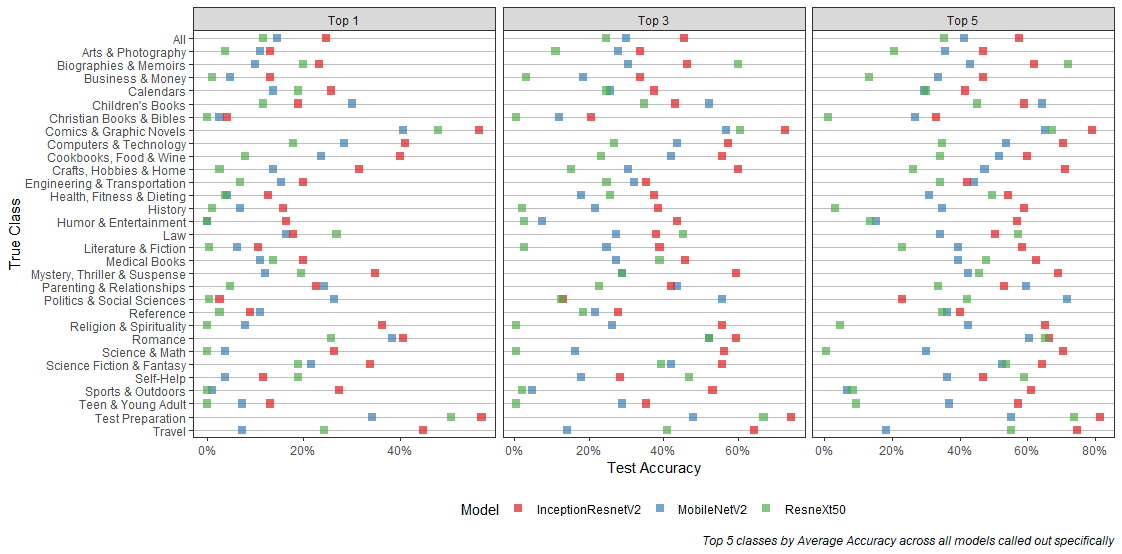
\includegraphics[scale=0.5]{accuracy_by_model.png}
	\caption{Top-1/3/5 recall (accuracy for all) of each model by genre}
	\label{fig:test_perf}
\end{figure}

\begin{table}[]
	\centering
	\resizebox{\textwidth}{!}{%
	\begin{tabular}{lrrr}
	\textbf{Predicted Genre}      & \multicolumn{1}{c}{\textbf{MobileNetV2}} & \multicolumn{1}{c}{\textbf{InceptionResnet-V2}} & \multicolumn{1}{c}{\textbf{ResNeXt50}} \\ \hline
	Arts \& Photography           & 17.8                                     & 20.8                                            & 25.9                                   \\
	Biographies \& Memoirs        & 11.5                                     & 19.3                                            & 5.5                                    \\
	Business \& Money             & 11.0                                     & 13.4                                            & 20.0                                   \\
	Calendars                     & 32.5                                     & 31.2                                            & 16.8                                   \\
	Children's Books              & 24.2                                     & 36.7                                            & 13.2                                   \\
	Christian Books \& Bibles     & 5.6                                      & 17.4                                            &                                        \\
	Comics \& Graphic Novels      & 19.7                                     & 46.5                                            & 17.1                                   \\
	Computers \& Technology       & 26.3                                     & 31.1                                            & 19.3                                   \\
	Cookbooks, Food \& Wine       & 19.1                                     & 65.0                                            & 16.3                                   \\
	Crafts, Hobbies \& Home       & 14.2                                     & 27.5                                            & 31.3                                   \\
	Engineering \& Transportation & 10.2                                     & 54.3                                            & 12.3                                   \\
	Health, Fitness \& Dieting    & 5.9                                      & 15.2                                            & 5.9                                    \\
	History                       & 13.5                                     & 20.3                                            & 66.7                                   \\
	Humor \& Entertainment        & 0.0                                      & 13.4                                            & 0.0                                    \\
	Law                           & 16.1                                     & 24.1                                            & 9.4                                    \\
	Literature \& Fiction         & 8.7                                      & 11.6                                            & 50.0                                   \\
	Medical Books                 & 12.4                                     & 16.5                                            & 12.5                                   \\
	Mystery, Thriller \& Suspense & 25.8                                     & 23.8                                            & 19.5                                   \\
	Parenting \& Relationships    & 9.8                                      & 33.9                                            & 8.2                                    \\
	Politics \& Social Sciences   & 5.5                                      & 11.1                                            & 5.3                                    \\
	Reference                     & 19.4                                     & 26.2                                            & 10.2                                   \\
	Religion \& Spirituality      & 9.6                                      & 16.7                                            &                                        \\
	Romance                       & 14.6                                     & 44.0                                            & 14.0                                   \\
	Science \& Math               & 11.9                                     & 11.8                                            & 0.0                                    \\
	Science Fiction \& Fantasy    & 18.3                                     & 39.5                                            & 13.6                                   \\
	Self Help                     & 12.3                                     & 22.9                                            & 7.2                                    \\
	Sports \& Outdoors            & 22.2                                     & 26.0                                            & 0.0                                    \\
	Teen \& Young Adult           & 9.5                                      & 14.2                                            & 0.0                                    \\
	Test Preparation              & 50.4                                     & 43.7                                            & 13.0                                   \\
	Travel                        & 50.0                                     & 17.3                                            & 8.3                                    \\ \hline
	\textbf{Total Precision}      & \textbf{14.6}                            & \textbf{24.7}                                   & \textbf{11.7}                          \\ \hline
	\end{tabular}%
	}
	\caption{Top-1 Per class and total precision for each model}
	\label{tab:test_prec}
	\end{table}

% section Results end 
\subsection{Further Analysis} 
\label{sub:Further_Analysis} 
In the paper by Iwana they discuss the potential reasons for the disparity between the recall by genre and investigate some examples. They call out consistency of colour, objects, and text styles are key elements that impact the ability for a genre to be able to be predicted well by their models. Here we focus on the colour component as the strongest driver for predictability and investigate the ways in which the models may be driven by colour of the cover images.

First, as displayed in \cref{fig:col_distributions}, we can see that whilst there is a wide range of average RGB values and width/aspect ratio (height is almost entirely consistent across genres), there are no standout values in colour alone that allow for easy genre classification. Width/aspect ratio, something that wasn't directly included in the model (but was indirectly by the use of the padding applied during the pre-processing), contains some clearer distinctions; in particular Calendars have a very different distribution of aspect ratios compared to other genres, and children books contains some of the more wider books than many other categories. Whilst none of this alone would be enough to provide good classification, it does suggest that explicit inclusion of dimensional information in a model could improve the performance when combined with the existing output. 

\begin{figure}
	\centering
	\captionsetup{justification=centering}
	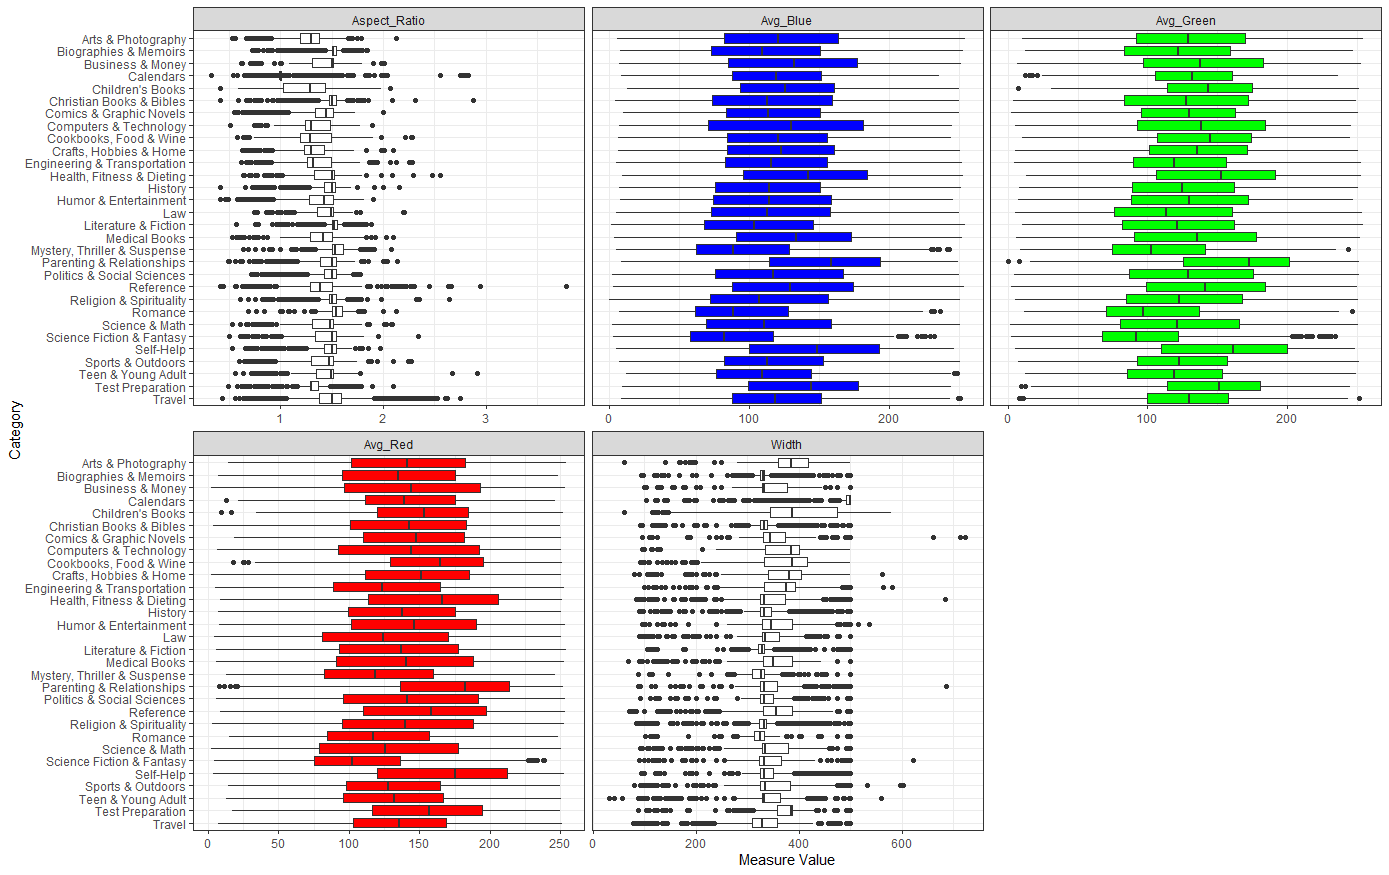
\includegraphics[scale=0.45]{distributions_col_ratio.png}
	\caption{Distributions of various measures by genre}
	\label{fig:col_distributions}
\end{figure}

The average overall colour per genre is presented in \cref{fig:avg_col} which does suggest some slight differences between the genres; similar to the callouts made by Iwana, Sci-Fi and Fantasy seem to be darker when compared to something like Cookbooks, Food and Wine. We can compare the average colour of the true classes vs those predicted by each model and visualise how these correlate with the recall per class as shown in \cref{fig:col_distance}. Here the colour distance is defined as 

\begin{equation}
	d_{colour} = \sqrt{(R_2 - R_1)^2 + ((G_2 - G_1)^2 +((B_2 - B_1)^2 }
\end{equation}
where R/G/B are the average red, green, and blue values for each predicted and class respectively. We can see a small trends here, particular in MobileNetV2, where the closer the average colour of the true class the better the recall of that class. This is of course a somewhat self-fulfilling prophecy; the more you correctly predict the class the more the dataset will be the true class, however is highlights that even by just guessing based on closeness to average colour you can make some small improvements. This supports the claims made by Iwana in their work. 


\begin{figure}
	\centering
	\captionsetup{justification=centering}
	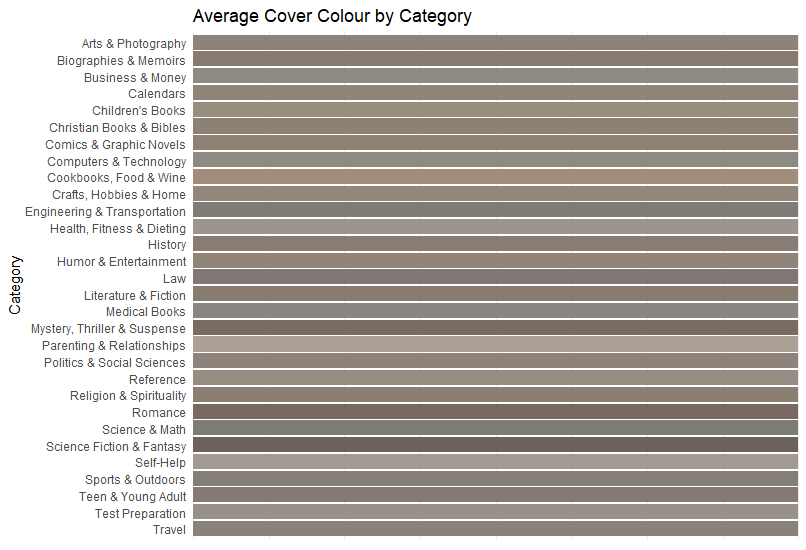
\includegraphics[scale=0.45]{avg_col_plot.png}
	\caption{Average cover colour by genre}
	\label{fig:avg_col}
\end{figure}

\begin{figure}
	\centering
	\captionsetup{justification=centering}
	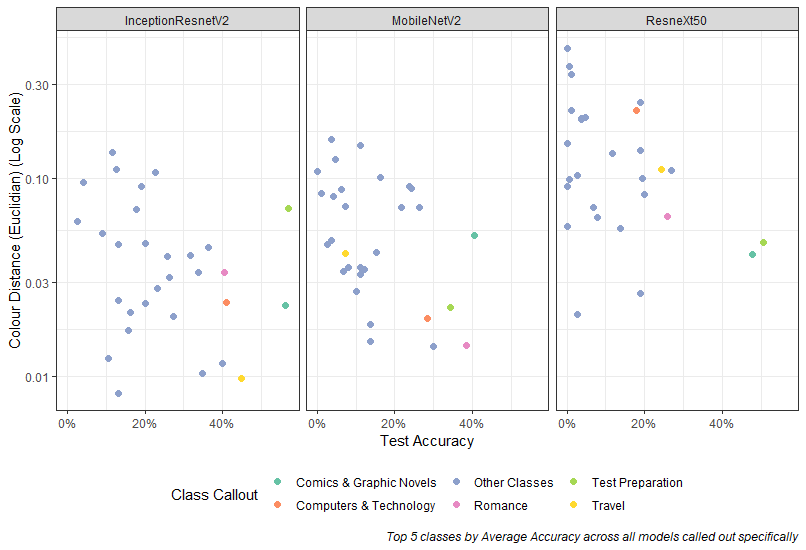
\includegraphics[scale=0.6]{col_dist_plot.png}
	\caption{Colour Distance vs Recall per genre by model}
	\label{fig:col_distance}
\end{figure}

Finally, we can review the \emph{class overlap} for each model. We define class overlap between class A and B for a single prediction as the ratio of the probability of prediction for class A and class B (where A has a higher probability) i.e.
\begin{equation}
	CO(A, B) \stackrel{\mathrm{def}}{=} \min\left\{\frac{P(A)}{P(B)}, \frac{P(B)}{P(A)}\right\}
\end{equation}
The per genre pair class overlap is defined as the average class overlap across all predictions. As we can see in \cref{fig:class_overlap}, where only class overlaps of greater than 0.5 are displayed, the ResNeXt50 model sees large amounts of class overlap between many classes, which agrees with what we saw before that certain classes were being \emph{confused} for each other by the model. Comparatively, MobileNetV2 sees only a few class overlaps greater than 0.5 and Inception-ResnetV2 sees none. When we examine those with higher overlap in MobileNetV2 we can begin to understand the potential true overlap between classes; Self-Help has overlap with Health, Fitness and Dieting, Science and Maths has overlap with Medical Books, and Religion and Spirituality has overlap with Christian Books and Bibles. All of these are logical overlaps and were a human tasked with classifying books based on their cover into these categories it is highly probable that different people would classify them differently. 

\begin{figure}
	\centering
	\captionsetup{justification=centering}
	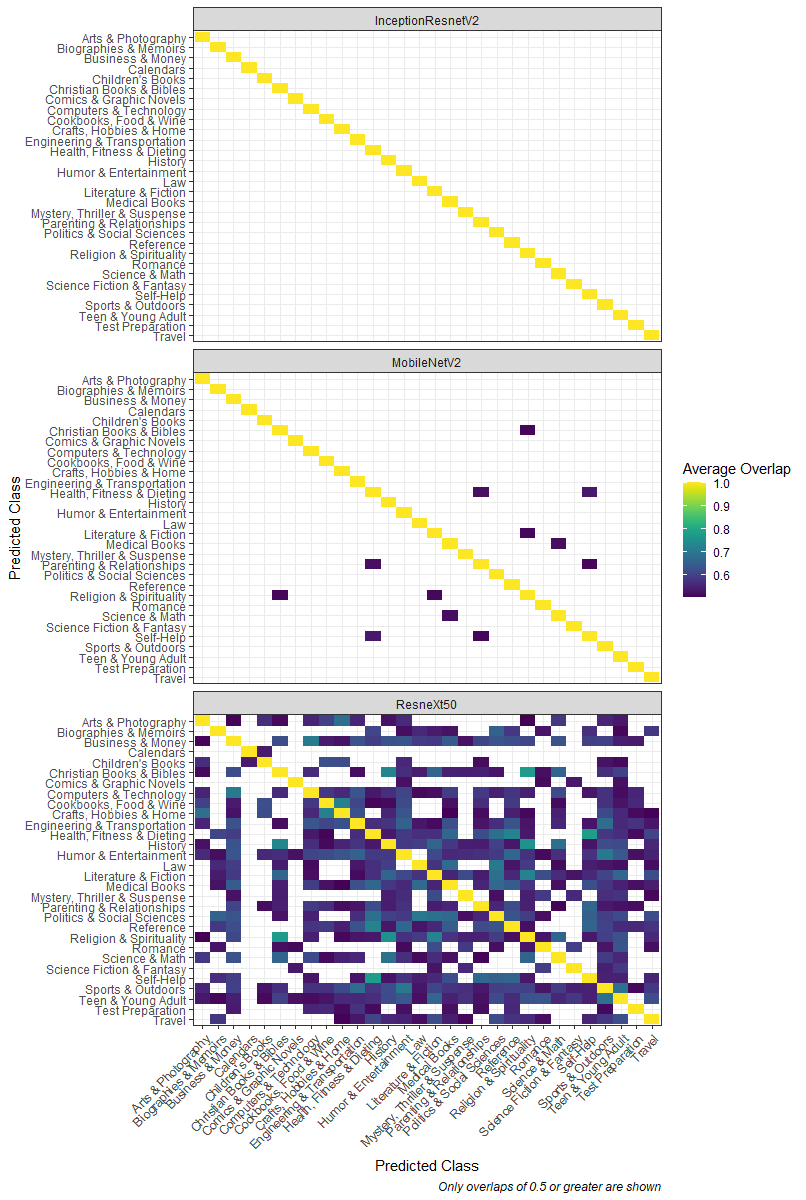
\includegraphics[scale=0.6]{class_pred_overlap.png}
	\caption{Average class overlap by model}
	\label{fig:class_overlap}
\end{figure}
% section Further_Analysis end 
\subsection{Feature Visualisation} 
\label{sub:Feature_Visualisation} 
The goal of using feature visualisation was to attempt to understand what, if any, underlying structure or information the models were using to aid their classification. To do this we use activation maximisation as implemented into the python package \emph{keras-vis}\cite{keras-vis} to do all the work. To produce the images the final layer activation function was changed from softmax to linear to ensure that class is being visualised as opposed to minimising other classes, and the loss function is simply defined as that linear activation (note here that loss is really a misnomer as we are trying to maximise this value as opposed to minimise it as we traditionally would) as discussed in \cref{sub:Activation_Maximisation}. L2 normalisation was used as the default to attempt to avoid pure static images being produced.

We ran the activation maximisation on the Inception-ResnetV2 model for the 3 best predicted genres (Test Prep, Comics \& Graphic Novels, and Travel) as we believed these had the best probability of returning useful images. The inputs to the model were then trained for 1000 epochs, at which point issues were encountered with the RAM on the machine. During these steps there was some improvement to the loss function however did not appear to converge and when compared to the progress seen on a pure imagenet model these saw very little movement and remained negative the entire time (where as the examples provided by the package are always positive after the first few epochs). 

The results of this attempt can be seen in \cref{fig:act_max_output} and whilst it may be possible to argue that there are some differences between these images that you could prescribe to the common layout of these type of genres covers, it would be difficult to say this with any conviction. Overall the images are generic and provided no additional insight to understand what features the model is identifying to use for the classification.

\begin{figure}
	\centering
	\captionsetup{justification=centering}
	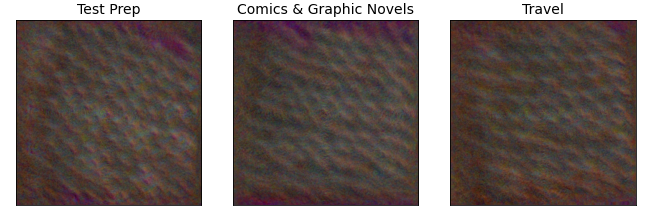
\includegraphics[scale=0.6]{visualize-dense-layer.png}
	\caption{Activation maximisation outputs for the 3 best predicted classes of the Inception-ResnetV2 model}
	\label{fig:act_max_output}
\end{figure}
% section Feature_Visualisation end  

\subsection{Discussion \& Future Work} 
\label{sub:Discussion} 
Overall the Inception-ResnetV2 model provided the best results of the 3 models we tried, however it is far more complex than AlexNet but did not provide greatly improved results. The counterpoint to this is that the AlexNet model as trained by Iwana et al was trained for 450,000 epochs where out model was trained for less than 50 epochs total. We do not know the progress of the training of the model by Iwana but it would be reasonable to suggest that if their model had trained for less epochs, or ours for more, then there would be a greatly difference between the results. Despite training on slightly less data (due to the validation set), we can see that more modern and powerful CNNs are able to predict book genres with slightly improved accuracy compared to older methods.

There are lots of directions this work could continue to go in the future; as mentioned before there is still more investigation that can be done surrounding the pre-processing of data, either varying the interpolation methods for downsizing or re-testing the pre-processing methods used specifically on the end model architecture for a longer period of time. Our models could be trained for more epochs with a greater requirement on early stopping to allow for long term improvements to be made that may not be evident over a few hundred epochs. Also, additional information such as the width and height or just aspect ratio could be passed to the model as well in an attempt to improve accuracy this way. The final fully connected part of the network could also be increased in complexity to contain more layers as opposed to just the single layer used in our work.

If resources were no constraint some of the larger improvements to the work would be to tune the hyperparameters of the model, and even train the actual core part of the architecture itself rather than relying entirely on transfer learning and freezing the weights for this component. To do this would require a far greater dataset of images so a generator may have to be used or a larger dataset collected first. Finally, as shown by the results in \cref{tab:results_acc} there is not a single model that performs best across all genres, so an ensemble method may be able to increase the accuracy at the cost of increased complexity. Many of these suggestions are beyond the scope of many citizen data scientists resources and would also lead to a model that may have a prediction time that makes it prohibitive for any real-time use.
% subsection Discussion end 
% section Evaluation_and_Further_Exploration end 

\section{Conclusion} 
\label{sec:Conclusion} 
In this work we have attempted to improve on the work by Iwana et al and better answer the question can a CNN judge a book by its cover. We reprocessed the dataset initially collected by Iwana and applied multiple pre-processing techniques in an attempt to identify the best method to deal with the impact of different shaped images. We then proceeded to train 3 modern models via transfer learning on a padded version of the dataset and evaluated the results. Finally we attempted to produce ideal class images using activation maximisation for the best model and genres.

We have seen that using a more modern CNN architecture, namely Inception-ResnetV2, we are able to improve on the results published by Iwana slightly whilst training for substantially less epochs. We have also provided some further supporting insight into the components that factor into book cover design i.e. colour, and identified where classifications are failing where this might be due to overlap between classes.

There is still lots to explore in this space as we discussed in \cref{sub:Discussion} and hopefully this work provides a springboard to enable more complex CNNs to be used for genre identification of book covers in the future. The work itself is unlikely to provide any value for real-world use as the accuracy is too low to be of use for either consumers or even cover designers as a form of QA. Genre prediction from cover images remains a complex topic and given the subjectivity of the classifications is unlikely to ever be fully solved, however the work produced here gets a little closer than we were before. So it seems for now that, if you are a CNN, you should follow the original advice and not try to judge a book by its cover.
% section Conclusion end 

%\nocite{*}
\bibliographystyle{ieeetran}
\bibliography{BBK_MSc_Project} 

\appendix

\section{CNN Architectures} 
\label{sec:CNN_Architectures} 
Detail the exact configurations of these architectures
\subsection{MobileNetV2} 
\label{sub:MobileNetV2} 
 
% subsection MobileNetV2 end  
\subsection{Inception-ResnetV2} 
\label{sub:Inception-ResnetV2} 
 
% subsection Inception-ResnetV2 end 
\subsection{ResNeXt50} 
\label{sub:ResNeXt50} 
 
% subsection ResNeXt50 end 
% section CNN_Architectures end 

\section{Technology} 
\label{sec:Technology} 
List of software and packages/libraries including their versions.
% section Technology end 
\end{document}